\documentclass[ngerman,a4paper,parskip=half]{scrartcl}

\usepackage[ngerman]{babel}
\usepackage[utf8]{inputenc}
\usepackage[onehalfspacing]{setspace}

\usepackage{helvet}
\usepackage[T1]{fontenc}
\usepackage{amsmath, amssymb, amstext}
\usepackage[affil-it]{authblk}
\usepackage[round]{natbib}
\usepackage[nolist,footnote]{acronym}
\usepackage{wrapfig}
\usepackage{fancyref}
\usepackage{graphicx}
\usepackage{xcolor}

\usepackage[hidelinks]{hyperref}
%\usepackage[left=3cm,right=4cm,top=3cm,bottom=6cm,includeheadfoot]{geometry}

\def \N{\mathbb{N}}
\def \Z{\mathbb{Z}}
\def \Q{\mathbb{Q}}
\def \R{\mathbb{R}}
\def \C{\mathbb{C}}
\def \fov{\mathrm{fov}}

\begin{acronym}[FOV]
	\acro{FOV}{Field of view}
\end{acronym}

\hypersetup{
	pdftitle    = {Streifenlichtprojektion und optische Analyse zur Oberflächeninspektion},
	pdfsubject  = {Streifenlichtprojektion},
	pdfauthor   = {Dennis~Wagner, Johannes~Spangenberg, Leroy~Kramer},
	pdfkeywords = {Streifenlichtprojektion, Humboldt, HU, Informatik},
	%	pdfcreator  = {pdflatex},
	%	pdfproducer = {LaTeX with hyperref},
}

%Kopf- und Fußzeile
\usepackage{fancyhdr}
\pagestyle{fancy}
\fancyhf{}

%Kopfzeile links bzw. innen
\fancyhead[L]{\nouppercase{\leftmark}}
%Kopfzeile rechts bzw. außen
\fancyhead[R]{\today}
%Linie oben
\renewcommand{\headrulewidth}{0.5pt}

%Fußzeile mittig
\fancyfoot[C]{\thepage}
%Linie unten
\renewcommand{\footrulewidth}{0.5pt}

\begin{document}

% ---------------------------------------------------------------------------- %

\definecolor{HUblue}{RGB}{0, 55, 108}

\begin{titlepage}
\begin{center}

%\colorbox{HUblue!30}{
\begin{minipage}{\textwidth}
	\begin{minipage}[c]{.8\textwidth}
		\textsc{\LARGE Humboldt-Universität zu Berlin}
		
		Institut für Informatik\\
		Lehrstuhl Signalverarbeitung und Mustererkennung
	\end{minipage}\hfill
	\begin{minipage}[c]{.2\textwidth}
		\includegraphics{husiegel}
	\end{minipage}
\end{minipage}
%}
\vspace{1.5cm}

\textsc{\Large Semesterprojekt}\\[0.5cm]

% Title
\newcommand{\HRule}{\rule{\linewidth}{0.5mm}}
\HRule \\[0.4cm]
{\huge \bfseries Streifenlichtprojektion und optische Analyse zur Oberflächeninspektion}
\HRule \\[1.5cm]

% Author and supervisor
\begin{minipage}{0.4\textwidth}
\begin{flushleft} \large
\emph{Autoren:}\\
Dennis~Wagner,\\
Johannes~Spangenberg,\\
Leroy~Kramer
\end{flushleft}
\end{minipage}
\hfill
\begin{minipage}{0.4\textwidth}
\begin{flushright} \large
\emph{Betreuende Hochschullehrerin:} \\
Prof.~Dr.~Meffert
\end{flushright}
\end{minipage}

\vfill

% Unterer Teil der Seite
{\large \today}

\end{center}
\end{titlepage}

\tableofcontents
\newpage

% ---------------------------------------------------------------------------- %

\section{Einleitung}

In verschiedenen Fällen ist es hilfreich oder notwendig ein \emph{komplexes} dreidimensionales Objekt zu vermessen. Aus solchen Vermessungen resultierende Modelle können in der Unterhaltungsindustrie für die Film- und Spielproduktion verwendet werden. Außerdem ermöglichen Verfahren zur Vermessung von Geometrien automatisierte Qualitätskontrollen und neue Methoden zur automatisierten Fertigung oder Verarbeitung.

In unserem Projekt arbeiten wir mit der \emph{Streifenlichtprojektion}. Dabei projizieren wir einen Streifen auf eine Oberfläche und rekonstruieren aus einer Aufnahme der projizierten Linie die Form der Struktur.

% ---------------------------------------------------------------------------- %

\section{Theoretische und technische Grundlagen}

Es haben sich in den letzten Jahrzehnten viele verschiedene Methoden entwickelt, mit denen man dreidimensionale Strukturen der realen Welt vermessen kann. So existieren zusätzlich zur Streifenlichtprojektion beispielsweise Verfahren, die \emph{Stereo-Vision}, \emph{Structure from Motion}, \emph{Shape from Shading} und \emph{Time of Flight} verwenden.

\subsection{Normalisierte Bildkoordinaten}
\label{sec:imagecoordinates}

Ein Bild besteht aus einer zweidimensionalen Matrix, die für jeden Pixel eine Farbe definiert. Bei der Verwendung der Indices der Matrix als Koordinaten für die Pixel stößt man schnell auf das Problem, dass die Lage des Pixels erst im Zusammenhang mit der Auflösung erkannt werden kann. Aus diesem Grund verwenden wir für unser Verfahren \emph{normalisierte Bildkoordinaten}. Das Ziel der normalisierten Koordinaten ist es, ohne Informationen über die Auflösung die Position eines Pixels auf der Bildebene ausdrücken zu können.

Als normalisierte Bildkoordinaten wird hier daher ein Tupel aus zwei reellen Zahlen $(u,v)$ verwendet. $v$ ist dabei aus dem Intervall $[-1,1]$. Der Wertebereich von $u$ ergibt sich entsprechend aus dem Seitenverhältnis $r$: $u \in [-r,r]$.

Um aus den Indizes $(i,j)$ eines Pixels die normalisierten Bildkoordinaten $(u,v)$ zu berechnen, kann folgende Gleichung verwendet werden:
\[ \begin{pmatrix}
u \\ v
\end{pmatrix} = 2 \cdot \begin{pmatrix}
\frac{i r}{s_x - 1} \\
\frac{j}{s_y - 1}
\end{pmatrix} - \begin{pmatrix}
r \\ 1
\end{pmatrix} \]
Mit der Bildauflösung $(s_x, s_y)$ und dem Seitenverhältnis $r = s_x/s_y$.

\subsection{Perspektivische Projektion}

Bei einer \emph{perspektivische Projektion} werden dreidimensionale Punkte auf eine \emph{Bildebene} projiziert. Die Funktion entsprechen dabei dem Modell der \emph{Lochkamera} und stellt eine Vereinfachung vieler realen Kameras da. Eine perspektivische Projektion wird durch den Augpunkt $O$ und die Bildebene definiert. Um einen Objektpunkt $X$ auf einen Punkt $X'$ in der Bildebene zu projizieren, bestimmt man den Schnittpunkt einer \emph{Projektionsgeraden} durch $X$ und $O$ mit der Bildebene. Den projizierten Punkt $X'$ nennt man auch \emph{Bildpunkt}. Im Gegensatz zur Lochkamera wird in schematischen Darstellungen die Bildebene meist zwischen Augpunkt und Objektpunkt dargestellt.

Oft verwendet man die perspektivische Projektion in Verbindung mit Bildern, wie sie in \Fref{sec:imagecoordinates} definiert werden, und nicht mit konkreten Bildpunkten. Dabei ist es meistens unwichtig, wo sie die Bildebene genau befindet, solange man jedem Pixel des Bildes genau eine Projektionsgerade zuordnen kann. Diese Zuordnung kann über die \emph{Focal length} $f$, dem Abstand zwischen Bildebene und Augpunkt, definiert werden. Seien $(u,v)$ normalisierte Bildkoordinaten eines beliebigen Pixels, so sieht die zugehörige Projektionsgerade G folgendermaßen aus:
\[ G = \left\lbrace \vec{w} \in \R^3 \middle\vert w = r \cdot \begin{pmatrix}
u \\ v \\ -f
\end{pmatrix} \land r \in \R \right\rbrace \]

%Da die Position der Bildpunkte in einem eigenen zweidimensionalen Koordinatensystem angegeben werden, benötigten wir noch Informationen zur Position der Bildebene in der Szene. Außerdem benötigen wir Informationen zur Skalierung der Koordinaten. Die Ausrichtung der Bildebene ist bereits durch die Rotation der Kamera gegeben. Eine Möglichkeit die restlichen benötigten Informationen zu definieren ist die Angabe der \emph{Focal length} $f$ und der Ausmaße der \emph{Bildebene}. Die Focal length ist die Entfernung der Bildebene vom Augpunkt. Wir gehen davon aus, dass die Bildpunkte in einem begrenzten Wertebereich liegen und betrachten die Ausmaße des entsprechenden Wertebereiches auf der Bildebene als die Ausmaße der Bildebene. Außerdem gehen wir davon aus, dass sich der Bildpunkt $(0,0)$ in der Mitte des Wertebereichs befindet und sich der entsprechende Punkt auf der Bildebene am nächsten am Augpunkt befindet.

%Da sich die Projektion bei proportionalen Änderungen der drei Werte nicht ändert, kann die Projektion bereits durch zwei der drei Werte beschrieben werden, indem man einen der drei Werte fest definiert. Eine äquivalente Möglichkeit zur Definition der Projektion ist die Angabe des vertikalen und horizontalen \ac{FOV}.

%%Des weiteren wird die Funktion durch das vertikale und horizontale \ac{FOV} bestimmt. Statt das \ac{FOV} direkt anzugeben ist es auch möglich das \ac{FOV} indirekt durch die Angabe der \emph{Focal length} $f$ und der Ausmaße der \emph{Bildebene} $(u, v)$ zu bestimmen. Da sich das \ac{FOV} bei proportionalen Änderungen der drei Werte nicht ändert, kann das \ac{FOV} bereits durch zwei der drei Werte beschrieben werden, indem man einen der drei Werte fest definiert.

%Um aus $f$ und $v$ das vertikale \ac{FOV} zu bestimmen, kann folgende Gleichung benutzen werden:
%\[ \fov^H = 2 \cdot \arctan \left( \frac{v}{2 f} \right) \]
%Die Berechnung des horizontalen \ac{FOV} erfolgt analog mit $u$ statt $v$.

%Umgekehrt ist es auch möglich aus dem \ac{FOV} mögliche Werte für $f$, $u$ und $v$ zu bestimmen. Sei $c:(0,\Pi)^2 \to \R$ eine beliebige Funktion, so erhalten wir mit den folgenden Berechnungsvorschriften gültige Werte für $f$, $u$ und $v$:
%\begin{align*}
%f &:= c(\fov^V,\fov^H)\\
%u &:= c(\fov^V,\fov^H) \cdot 2 \tan\left(\frac{\fov^H}{2}\right)\\
%v &:= c(\fov^V,\fov^H) \cdot 2 \tan\left(\frac{\fov^V}{2}\right)
%\end{align*}

%Für ein beliebigen Objektpunkt $x = (x_1, x_2, x_3)$ und dem dazugehörigen Bildpunkt $x'$ gilt bei unseren Annahmen die folgende Gleichung:
%\[ x' = \frac{f}{2 x_3} \cdot \begin{pmatrix}
%u x_1\\v x_2
%\end{pmatrix} \]

%\[ x_1 = \frac{2 x_1' x_3}{u f} \]
%\[ x_2 = \frac{2 x_1' x_3}{v f} \]

\subsection{Triangulation}

\subsubsection{Modell und gegebene Werte}

Das hier verwendete Modell besteht im wesentlichen aus einer perspektivischen Projektion eines Objektpunktes $X$ auf eine Bildebene $B$, die parallel zur $x$-$y$-Ebene verläuft. Das Augpunkt liegt dabei im Koordinatenursprung $O$. Der Bildpunkt wird mit $X'$ bezeichnet. Das projizierte Licht wird durch eine Ebene $L$ dargestellt, die die Position des Projektors, das heißt den Projektionspunkt $P$, und den Objektpunkt $X$ schneidet.

Die durch das Setup gegebenen Werte:

\begin{tabular}{lp{12cm}}
	$P$       & Position des Linienprojektors.\\
	$f$       & Focal length (unter der Annahme, dass die Ausmaße der Bildebene zwei Einheiten nach oben betragen)\\
	$\theta$  & Winkel zur Ausrichtung des Projektors.\\
	$\delta$  & Zweiter Winkel zur Ausrichtung des Projektors.
\end{tabular}

Zudem ist der Bildpunkt durch normalisierte Bildkoordinaten $(u, v)$ gegeben. Da die Focal length $f$ auf eine Bildhöhe von zwei Einheiten angepasst ist, gilt $X'(u, v, -f)$.

\subsubsection{Bestimmung der Entfernung}

\begin{wrapfigure}{r}{6cm}
	\centering
	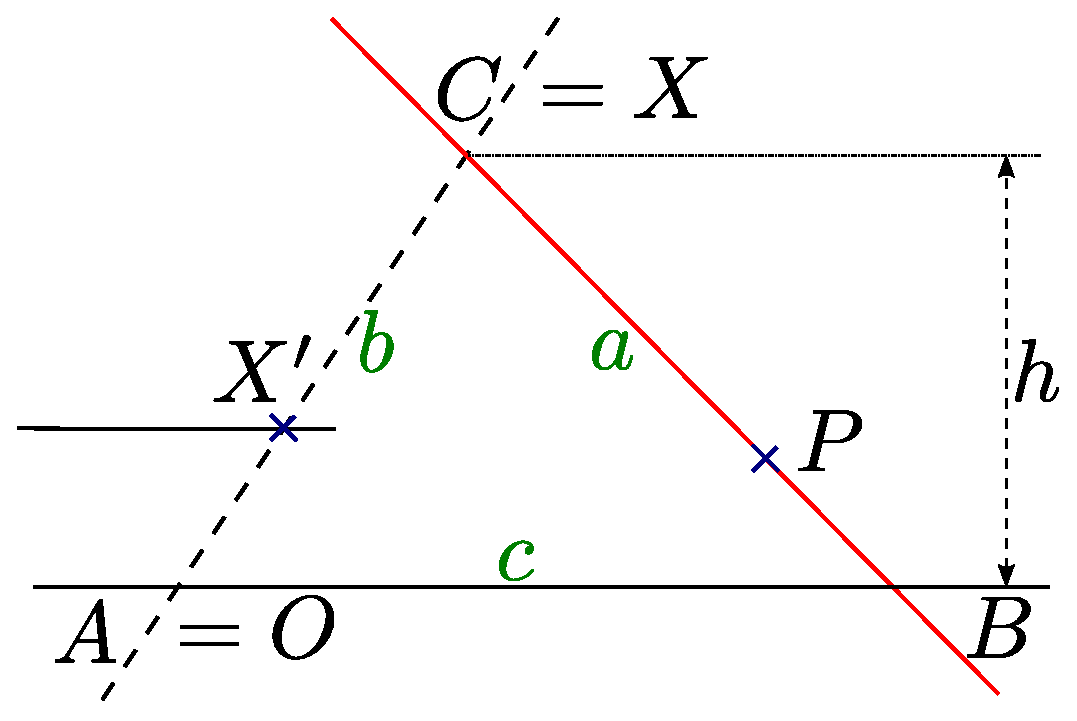
\includegraphics[width=\linewidth]{includes/triangulation2d}
	\caption{Zweidimensionales vereinfachtes Modell des Setups}
\end{wrapfigure}

Als \emph{Entfernung des Objektpunktes}, bzw. $h$, wird die 3. Koordinate von $X$ bezeichnet.

Um diese Entfernung zu bestimmen, wird das geometrische Modell des Setups vereinfacht. Als erstes wird ein Basiswechsel auf die Orthogonalbasis
\[ \left\lbrace \begin{pmatrix}
\cos(\theta) \\ \sin(\theta) \\ 0
\end{pmatrix}, \begin{pmatrix}
0 \\ 0 \\ -1
\end{pmatrix}, \begin{pmatrix}
\sin(\theta) \\ \cos(\theta) \\ 0
\end{pmatrix} \right\rbrace \]
vorgenommen, um im folgenden nur die ersten beiden Dimensionen zu betrachten. Der konstruierte zweidimensionale Raum hat die besondere Eigenschaft, dass von der Ebene $L$ und der $x$-$y$-Ebene nur die Geraden $a$ und $c$ übrig bleiben. Eine weitere besondere Eigenschaft ist, dass der Abstand zwischen $X$ und der $x$-$y$-Ebene direkt von einen in den anderen Raum übernommen werden kann. Ein beliebiger Vektor $(v_1, v_2, v_3)^T$ im dreidimensionalen Model entspricht damit im zweidimensionalen Modell dem Vektor $(\cos(\theta) \cdot v_1 - \sin(\theta) \cdot v_2, -v_3)^T$.

Die Geraden $a$ und $c$ bilden zusammen mit der Geraden $b$, welche durch die Punkte $O$, $X$ und $X'$ verläuft, ein Dreieck, dessen Eckpunkte $A$, $C = X$ und $B = O$ sind. Angenommen die Koordinaten von $P$ und $X'$ in der zweidimensionalen Darstellung sind $(p_1,p_2)$ und $(x'_1, x'_2)$, so können die Winkel $\alpha$ und $\beta$ und die Länge der Strecke zwischen $A$ und $B$ wie folgt berechnet werden:
\begin{align*}
	\alpha &= \frac{\pi}{2} - \arctan\left(\frac{x'_1}{x'_2}\right)\\
	\beta &= \frac{\pi}{2} + \delta\\
	\overline{AB} &= p_1 + \tan(\delta) \cdot p_2
\end{align*}

Die Entfernung $h$ kann nun über die folgende Gleichung berechnet werden:
\[ h = \frac{\overline{AB} \cdot \sin(\alpha) \cdot \sin(\beta)}{\sin(\pi - \beta - \alpha)} \]

\subsubsection{Bestimmung der Koordinaten}

Die Koordinaten des Objektpunktes X in unserem Modell können durch die folgende Gleichung berechnet werden:
\[ \vec{x} = \frac{h}{f} \cdot \begin{pmatrix}
u \\ v \\ -f
\end{pmatrix} \]

% ---------------------------------------------------------------------------- %

\section{Aufbau und Algorithmen}

\subsection{Hardware}

Die Hardware besteht aus einer Webcam und einem Linienlaser, der auf einem Modellbauservo montiert ist. Laser und Servo werden von einem ''Spark Core'' Mikrocontroller gesteuert, welcher wiederum über USB von der Software gesteuert wird.

\subsection{Grundlegende Softwarearchitektur}

\subsection{Klassen und Funktionsüberblick}

\subsection{Ansteuerung der Hardware}

Die Software steuert die Hardware über USB, wobei sich der Mikrocontroller als virtuellen COM-Port ausgibt. Zur Kommunikation wird ein einfaches Protokoll verwendet, das 2 Byte lange Nachrichten an den Mikrocontroller sendet. Das erste Byte gibt den Befehl an, das zweite den Parameter.\\

\begin{tabular}{|c|c|c|}
\hline
1. Byte & 2. Byte & Beschreibung \\
\hline
'm'\footnotemark & $\alpha \in [0,180]$ & Setzt die Servoposition auf $\alpha ^\circ$.\\
\hline
'l' & '0' oder '1' & Schaltet den Laser an ('1') bzw. aus ('0')\\
\hline
\end{tabular}

\footnotetext{Zeichen in Anführungszeichen stehen für den ASCII-Wert des Zeichens}


\subsection{Linienerkennung}

Es wird ein Binärbild erzeugt, wobei der Algorithmus entscheidet, welche Pixel zur Linie gehören und welche nicht. Im zweiten Schritt wird das Bild zeilenweise durchgegangen, wobei in eine seperate Datenstruktur die vermeintliche Position der Linie und deren Breite geschrieben wird. Diese Informationen werden dann an die Auswertungssoftware weitergegeben. Die hier implementierten Algorithmen unterscheiden sich lediglich in der Erzeugung des Binärbildes im ersten Schritt.

\subsubsection{Differenzbildung (Diff)}

Vor der eigentlichen Aufnahme mit dem Laser oder nach jeder einzelnen Aufnahme wird ein Bild ohne eine Linie aufgenommen. Mit jedem weiteren Bild wird die Differenz mit der Aufnahme ohne Linie gebildet und mit Hilfe einer Maske wird das Rauschen entfernt und das Bild in ein Binärbild umgewandelt.

\subsubsection{Farbfilter (Free)}

Für jeden Farbkanal wird einzeln der Mittelwert über das gesamte Bild berechnet, aus dem ein Schwellenwert für jeden Kanal einzeln bestimmt wird. Für jeden Pixel wird der Wert jedes Farbkanals mit dem Schwellenwert verglichen. Ist ein Wert keiner als der entsprechnde Schwellenwert, gehört der Pixel nicht zur Linie.

\subsection{Rekonstruktion}

% ---------------------------------------------------------------------------- %

\section{Auswertung}

% ---------------------------------------------------------------------------- %

\section{Zusammenfassung}

% ---------------------------------------------------------------------------- %

\section{Quellenverzeichnis}

% ---------------------------------------------------------------------------- %

\end{document}
